% 1. ročník MAT – příprava 97; inspirace Realisticky.cz 020501–020506, úlohy nově sestavené.
\documentclass[11pt,a4paper]{article}
\input{../../sablony/pripravy/priprava.sty}
\usepackage{tikz}
\usepackage{pgfplots}
\pgfplotsset{compat=1.18}
\usetikzlibrary{arrows.meta}
\nastavPripravu{1. ročník}{Kvadratické funkce}{97}{Kvadratická funkce y=ax²}
\begin{document}
\blok{Od jediné paraboly k celé rodině}
Známe $y=x^2$. Co se změní, když funkční hodnoty vynásobíme konstantou $a\ne0$? V každém grafu zůstává bod $[0;0]$, ale mění se orientace i „šířka“ paraboly.
\begin{definiceBox}
Pro $f(x)=ax^2$, $a\ne0$, platí: $a>0$ parabola míří vzhůru a $H(f)=\langle0;+\infty)$;
$a<0$ míří dolů a $H(f)=(-\infty;0\rangle$. Vrchol je vždy $V[0;0]$ a osa souměrnosti $x=0$.
Při větší hodnotě $|a|$ je parabola \emph{užší} než $y=x^2$, při $0<|a|<1$ \emph{širší} (ve stejném měřítku).
\end{definiceBox}
\begin{center}
\begin{tikzpicture}
\begin{axis}[
width=10cm,height=6.8cm,axis lines=middle,
xmin=-3.1,xmax=3.1,ymin=-6,ymax=8,
xtick={-3,-2,...,3},ytick={-6,-4,...,8},grid=both,
minor tick num=0,grid style={black!12},
tick label style={font=\scriptsize},xlabel={$x$},ylabel={$y$},
label style={font=\small},restrict y to domain=-6:8,
clip=true,legend style={font=\scriptsize,draw=none,fill=none,at={(0.98,0.98)},anchor=north east},
]
\addplot[very thick,solid,domain=-3.1:3.1,samples=160] {x^2};
\addlegendentry{$y=x^2$}
\addplot[very thick,dashed,domain=-3.1:3.1,samples=160] {2*x^2};
\addlegendentry{$y=2x^2$}
\addplot[very thick,dotted,domain=-3.1:3.1,samples=160] {0.5*x^2};
\addlegendentry{$y=\tfrac12x^2$}
\addplot[very thick,dash dot,domain=-3.1:3.1,samples=160] {-x^2};
\addlegendentry{$y=-x^2$}
\end{axis}
\end{tikzpicture}
\end{center}
\blok{Společně řešené příklady}

\begin{prikladReseniBox}
Porovnejte $f(x)=2x^2$, $g(x)=\tfrac12 x^2$ a $h(x)=-3x^2$: orientace, vrchol, obor hodnot a hodnoty v $x=2$.
\tcblower
\[
\begin{aligned}
f(2)&=8,\quad g(2)=2,\quad h(2)=-12 \\
H(f)&=H(g)=\langle0;+\infty) \\
H(h)&=(-\infty;0\rangle \\
V_f&=V_g=V_h=[0;0]
\end{aligned}
\]
První dvě paraboly mají minimum, poslední maximum; nejstrmější u osy je $h$.
\end{prikladReseniBox}
\begin{prikladReseniBox}
Kvadratická funkce $f(x)=ax^2$ prochází bodem $A[2;12]$. Určete $a$ a vypočtěte $f(-1)$.
\tcblower
\[
\begin{aligned}
12&=a\cdot2^2 \\
a&=3 \\
f(x)&=3x^2,\qquad f(-1)=3
\end{aligned}
\]

\end{prikladReseniBox}
\blok{Samostatné procvičování}

\begin{zadaniReseniBox}
a) Určete orientaci a obor hodnot $y=-\tfrac14x^2$.\par
b) Při $f(-3)=-18$ a $f(x)=ax^2$ určete $a$.\par
c) Uvažujte $y=ax^2$ s $a\in\{-2;\tfrac12;2\}$. Kolik různých grafů vznikne a které směřují dolů?
\tcblower
\[
\begin{aligned}
H&=(-\infty;0\rangle,\quad\text{parabola míří dolů} \\
-18&=9a\ \Rightarrow\ a=-2 \\
\text{Vzniknou }&3\ \text{grafy; dolů míří jen }a=-2.
\end{aligned}
\]

\end{zadaniReseniBox}
\blok{Krátká otázka k porozumění}
Lze najít $a\ne0$ tak, aby parabola $y=ax^2$ procházela bodem $[1;0]$? Ne: $0=a\cdot1$, takže by muselo platit $a=0$ a nešlo by o kvadratickou funkci.
\blok{Domácí úkol}
\begin{zadaniReseniBox}[title={Domácí příprava}]
\begin{enumerate}[label=\alph*),itemsep=3pt]
\item Pro $f(x)=3x^2$ dopočítejte $f(-2)$, $f(0)$ a $f(3)$.
\item Pro $g(x)=-2x^2$ určete $g(-1)$, $D(g)$, $H(g)$ a maximum.
\item Určete $a$, jestliže $f(x)=ax^2$ a $f(2)=20$.
\item Určete $a$, jestliže $f(x)=ax^2$ a $f(-3)=-9$.
\item Naskicujte v jedné soustavě $y=x^2$, $y=2x^2$ a $y=-x^2$; určete společný bod.
\item Pro $f(x)=-\tfrac12 x^2$ vyznačte vrchol, osu souměrnosti, intervaly monotonie a $H(f)$.
\item \textbf{Výzva:} Pro jaké $a\ne0$ leží bod $[4;-8]$ na grafu $y=ax^2$? Je graf širší než $y=x^2$?
\end{enumerate}
\tcblower
\begin{enumerate}[label=\alph*),itemsep=4pt]
\item
\[
\begin{aligned}
f(-2)&=12,\quad f(0)=0,\quad f(3)=27
\end{aligned}
\]

\item
\[
\begin{aligned}
g(-1)&=-2,\quad D(g)=\mathbb R \\
H(g)&=(-\infty;0\rangle,\quad \max g=0
\end{aligned}
\]

\item
\[
\begin{aligned}
20&=4a\ \Rightarrow\ a=5
\end{aligned}
\]

\item
\[
\begin{aligned}
-9&=9a\ \Rightarrow\ a=-1
\end{aligned}
\]

\item
\[
\begin{aligned}
[0;0]&\ \text{leží na všech třech grafech} \\
\text{Konstrukce }&\text{např. přes }x=\pm1,\pm2.
\end{aligned}
\]

\item
\[
\begin{aligned}
V&=[0;0],\quad\text{osa }x=0 \\
\text{roste na }&(-\infty;0\rangle,\ \text{klesá na }\langle0;+\infty) \\
H(f)&=(-\infty;0\rangle
\end{aligned}
\]

\item
\[
\begin{aligned}
-8&=16a\ \Rightarrow\ a=-\tfrac12 \\
0<|a|&=\tfrac12<1\ \Rightarrow\ \text{širší, míří dolů.}
\end{aligned}
\]

\end{enumerate}
\end{zadaniReseniBox}
\poznamka{Čas: společný obrázek 10 min, význam koeficientu 10 min, dva vedené příklady 12 min, samostatně 10 min, závěr 3 min. Učitel nemění měřítko jednotlivých grafů; jinak přímé porovnání šířek ztrácí smysl.}
\end{document}
